\documentclass[10pt]{article}
\usepackage[document]{ragged2e}
\usepackage{multicol}
\usepackage[margin=1in]{geometry}
\usepackage{titlesec}
\usepackage{fancyhdr}
\usepackage{graphicx}
\graphicspath{ {./images/} }
\usepackage[justification=centering]{caption}
\captionsetup[subfigure]{justification=centering}
\captionsetup[figure]{justification=centering}
\usepackage{subcaption}


\pagestyle{fancy}
\fancyhf{}
\fancyfoot[R]{Page. \thepage}
\fancypagestyle{plain}{
    \renewcommand{\headrulewidth}{0pt}
    \fancyhf{}
    \fancyfoot[R]{Page. \thepage}
}

\setlength{\parindent}{0em}
\setlength{\parskip}{1em}
\titlespacing*{\section}{0pt}{0.2em}{0.5em}
\titlespacing*{\subsection}{0pt}{0.2em}{0.2em}
\titlespacing*{\subsubsection}{0pt}{0.2em}{0.2em}


\title{Checkpoint 3: Interactive Visualization}
\author{The Freedom Deer: Tianchang Li, Hualiang Qin, Qingwei Lan}

\begin{document}
\maketitle


\textbf{The full analysis, along with the interactive plots, is shown in \\ https://observablehq.com/@c69ef2da2b4d284b/checkpoint-3-interactive-visualization}

Our group implemented three interactive visualizations in Observable. The first one is a bubble chart of the cross race situation of use of force cases along the time scale. The second one is a top k bar chart showing under what conditions of four different circumstances the use of force is more likely to occur. The third one is a sunburst that aims to portrait the subject and officer who are involved in the tactical response report.

\section{Bubble Chart view of the Cross Race Use of Force Cases}

Interactive plots are shown in \\ https://observablehq.com/@c69ef2da2b4d284b/bubble-plot-of-cross-race.

Example is shown in Figure \ref{bubbleplot-officer}.

\begin{figure}[h]
\centering
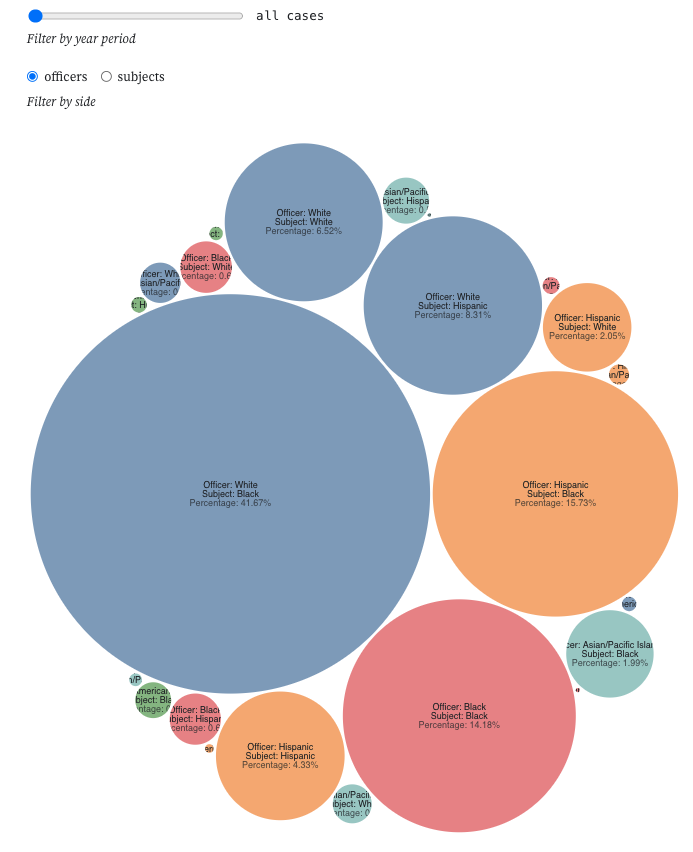
\includegraphics[scale=0.47]{bubbleplot-officer}
\caption{Example bubble plot showing use of force cases. Graph allows filtering by time period and by officer or subject.}
\label{bubbleplot-officer}
\end{figure}

\subsection{The Context}

Based on previous research, we have observed that the majority of the cross race use of force cases happened under the white officer and black subject combination. However, given the fact that the majority of policemen are white and the majority of subjects are black, the observed fact seems to be intuitive. Expecting new discoveries, we divided the data (2004-2016) into four pieces where each interval is either three years or four years. We are eager to see how the cross race use of force cases change along the time scale.

\subsection{The Data}

We queried the \texttt{trr\_trr} table in the CPDB database for the cross race situation (5 race of officer vs 5 race of subject). For each combination, we calculate the percentage of its occurrence of the total number of trr cases.

\subsection{How do the cross race use of force cases change every three years \\ from 2004 to 2016?}

As time went by, the majority of the cross race situation still happened under white police and black subject range from 40\% to 43\% among all the use of force cases. The top cross race use of force cases are white officer to black subject, hispanic officer to black subject, black officer to black subject, white officer to hispanic subject, and white officer to white subject. The fact that black subjects made up about 70\% of the total subjects and the white officers made up about 60\% of total officers doesn’t change over the years so does the top cross race situations.


\section{Bar Chart view of the Likelihood of use of force occurrence of each condition under 4 circumstances}

Interactive plots are shown in \\ https://observablehq.com/@c69ef2da2b4d284b/bar-chart-horizontal-environmental-factor-on-use-of-force.

Example is shown in Figure \ref{barchart}.

\begin{figure}[h]
\centering
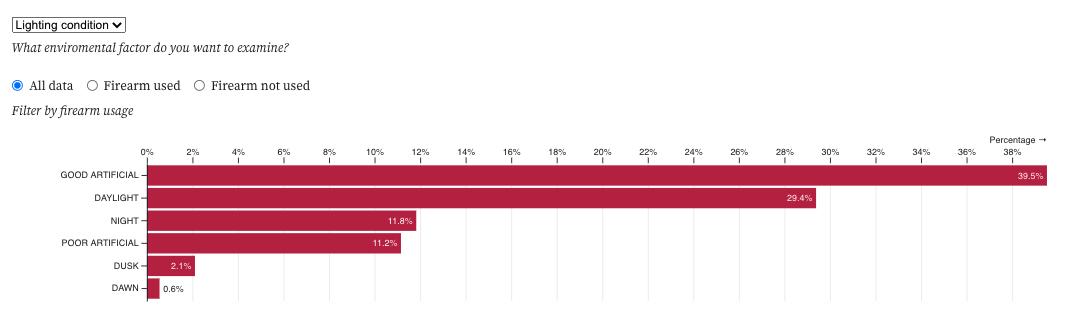
\includegraphics[scale=0.45]{barchart}
\caption{Example barchart showing all data for lighting conditions. The graph allows selection of different envirionmental factors and allows filtering by firearm usage.}
\label{barchart}
\end{figure}

\subsection{The Context}

In our previous research, we examined the occurrence of use of force cases under different conditions of 4 different circumstances (Lighting condition, Location, Weather, Indoor/Outdoor). We observed that the use of force cases are more likely to happen under the broad and bright situation. In this section, we want to see whether the usage of firearms would make a difference on what the chart looks like.

\subsection{The Data}

We queried the \texttt{trr\_trr} table in the CPDB database for each circumstance, and then we splitted the data under each circumstance by if firearms were involved.

\subsection{How does the likelihood change with respect to if firearms were involved?}

In terms of lighting conditions, the involvement of firearms didn’t change the top k conditions, however, the top one condition (good artificial light) made up more occurrences when firearms were involved. The percentage rose from 39\% to 48\%. This situation also happened under other circumstances. When firearms were involved, under indoor/outdoor scenario, the top one condition–outdoor rose from 70\% to 85\%; under different weather conditions, the top one condition–clear weather rose from 81\% to 89\%; under different locations, the top one condition–street rose from 27\% to 30\%. One thing that needs attention is that the percentage for street conditions didn’t rise that much, however, the 2nd-ranked condition–sidewalk was split by itself and the condition alley, while it is far beyond the ranked third condition when firearms are not involved.

From previous research, we concluded that the use of force usually happens under good circumstances which implies better sight and broader area. If we consider the usage of firearms as an escalation of the general use of force case, it is reasonable that it relied more on the ``good circumstances".


\section{Sunburst view that depicting subjects and officers}

Interactive plots are shown in \\ https://observablehq.com/@ltcrazy/sequence-sunburst-portraiting-the-demographics-of-the-2-pa.

Example is shown in Figure \ref{sunburst-subject} and Figure \ref{sunburst-officer}.


\begin{figure*}
\captionsetup{font=small}
    \begin{subfigure}{0.5\textwidth}
        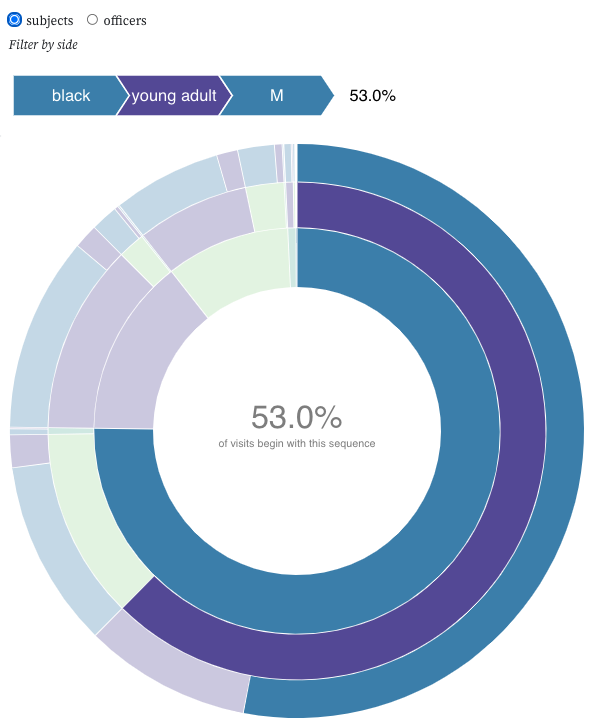
\includegraphics[width=\textwidth]{sunburst-subject}
        \caption{Sunburst for subjects}
        \label{sunburst-subject}
    \end{subfigure}%
    \begin{subfigure}{0.5\textwidth}
        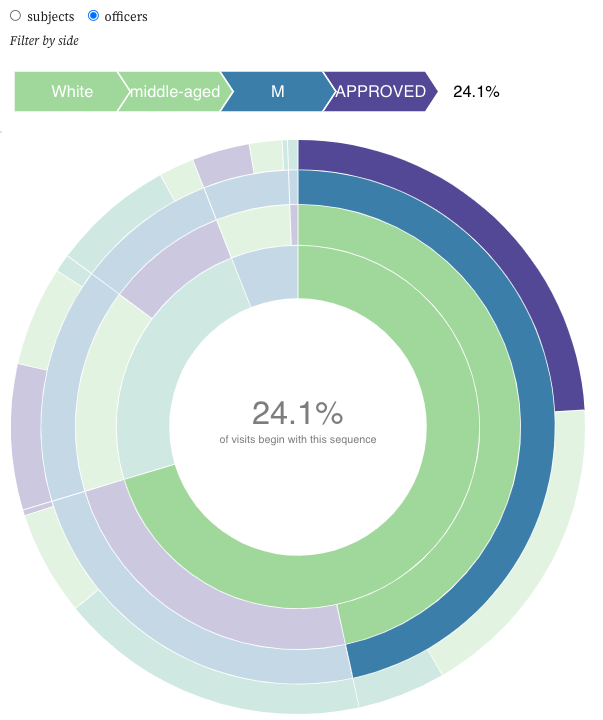
\includegraphics[width=\textwidth]{sunburst-officer}
        \caption{Sunburst for officers}
        \label{sunburst-officer}
    \end{subfigure}
\caption{Sunburst plots for officers and subjects. Hovering over the plots allows dynamic filtering.}
\end{figure*}

One of our primary goals for this project is to depict the groups of individuals who are most risky to the use of force and the groups of police officers who are most prone to exercise violence. To achieve this, we extracted demographic information of the subjects and officers joining \texttt{trr\_trr}, \texttt{trr\_trrstatus}, and \texttt{data\_officer} tables and plotted sunburst diagrams. The composition of race, age and gender is considered for both subjects and officers. Moreover, the TRR status is included in the officers' diagram.

\subsection{What did we observe from the sunburst?}

\begin{enumerate}

\item The sunburst diagram for subjects clearly illustrates that black population is the most risky to the use of force, that young adults (18-40 year-old) are the most risky to the use of force among all races, and that male subjects are the most common among all races and all age groups. Hispanic and white population come in second in terms of race. Middle-aged group comes in second in terms of age. Female subjects are rarer in all races and age groups.

\item The sunburst diagram for officers illustrates that white officers dominate the police officers involved in use of force cases, that middle-aged ($>40$ year-old) officers dominate in all race groups, and that males dominate in all race-age combinations. Although, let us not overlook the fact discovered earlier that most officers are white males. Young adults ($<40$ year-old) comes in second being very close to the middle-aged group for both white and hispanic officers.

Another interesting finding from this diagram is about the approval rate of TRR reports for different race and age groups. It is much more likely for black officers’ TRR reports to be approved than those of hispanic and white officers ($\frac{1}{2}$ vs. $\frac{1}{3}$). Besides, the officers in the middle-aged group have their TRR reports approved much more likely than those in the young-adult group (nearly none).

\end{enumerate}


\section{Conclusion and Future Direction}

To sum up, white and hispanic males between 18-40 year-old are the most risky to police’s use of force. We suggest these groups be aware of such facts and risks. White males and hispanic males older than 40 year-old are prone to exercise violence. We suggest more effective internal training on restraining use of force for these groups as well as their potential biases towards risky groups mentioned above. Among all officers, black officers older than 40 year-old are most likely to have their TRR approved. With this information, we suggest monitoring more closely on other police groups to encourage restraining use of force.

In terms of the circumstance of use of force occurrence, the fact that use of force is more likely to happen under the circumstance that has better sight and broader area needs to be noticed. More importantly, the TRR cases that involved usage of firearms relied more on this ``good circumstance". As a complementary of the suggestion mentioned above, we recommend those groups with higher risk of use of force be more conscious under the ``good circumstance".

In the future, more research can be done to explore the underlying mechanism of the occurrence of use of force from the perspective of the effect of aging and environmental implication. The difference of psychological status of the officers under certain circumstances and among different age groups could also be studied as the potential consideration of the risk of use of force.






\end{document}
